\subsection{封建女性地位}
\begin{frame}{“三从四德”下缺失自由和地位卑微}
    \begin{block}{周南·桃夭}
        \begin{verse}
            桃之夭夭,灼灼其华。之子于归,宜其室家。 \\
            桃之夭夭,有蕡其实。之子于归,宜其家室。 \\
            桃之夭夭,其叶蓁蓁。之子于归,宜其家人。 \\
        \end{verse}
    \end{block}
    \begin{block}{}
        \begin{itemize}
            \item “三从四德”、“女子无才便是德”
            \item 娘家教导女子成为淑女,遵守妇道,维护娘家形象,婆家检验女子是否具有妇德
            \item 为人妻前,遵从父母之命媒妁之言,娘家束缚她的思想;为人妻后,婆家延续对女性的管教,禁锢她的自由
        \end{itemize}
    \end{block}
\end{frame}

\begin{frame}{女性在人格与生活上的依附性}
    \begin{block}{《京华烟云》}
        \small
        孙曼娘是一个典型的传统女子形象。她一生都为她的丈夫亚平活着,哪怕只是一个拥抱,她便认定了他是亚平的人,即使男人病重也毅然决然的嫁给了他,并在亚平死后,坚持着“生是曾家人,死是曾家鬼”的信念而守活寡,哪怕在其拥有了养子后,又将生活重心放在了儿子身上,几乎没有真正的为自己独立的人格活过,始终将自己的人格依附在男人、家庭、孩子身上,更别说是生活了,恐怕自己一个人也是活不下去的。赫拉克利特说:“一个人的性格就是他的命运。”孙曼娘的悲剧就在于受到传统意识观念洗礼而丧失自我的依附性人格。
    \end{block}
    \begin{block}{《白鹿原》}
        \small
        田小娥无疑也是命运悲惨的女性形象代表 ,她自小被卖给能做她爷爷的郭举人做小妾,为了摆脱这种水深火热的生活状态,她主动依附于黑娃,在黑娃出走之后,又将活下去的希望寄托于白孝文的身上。生活与命运对于田小娥是不公平的,但在寻找出路的过程中,她本能的选择了“男人”,这种对男性的依附性使得她从不相信在那样的时代能够靠自己的努力活下去,而事实也证明了,她最终还是没能找到一个护她一世周全的男人,最终悲惨死去。
    \end{block}
\end{frame}



\subsection{近代女权思想的出现}
\begin{frame}{社会经济的发展}
    \begin{block}{}
        \begin{itemize}
            \item 小农经济时期:男人和女人在体质和体力上确实存在自然差异,这就有了男尊女卑的反映,女性受世俗观念的影响更是被禁锢在了家中;
            \item 民族资本主义:企业里上出现工作强度不太大但需要很细致地进行的一类工作,适合女性工人来进行生产。
        \end{itemize}
    \end{block}
    \begin{center}
        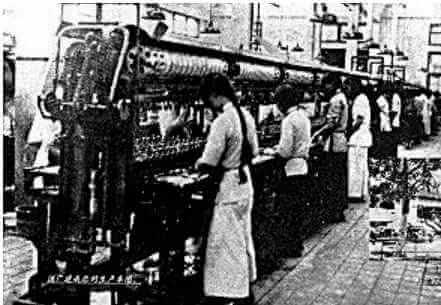
\includegraphics[width=.45\textwidth]{../docs/img/1-2.jpg}
    \end{center}
\end{frame}

\begin{frame}{社会经济的发展}
    \begin{figure}
        \centering
        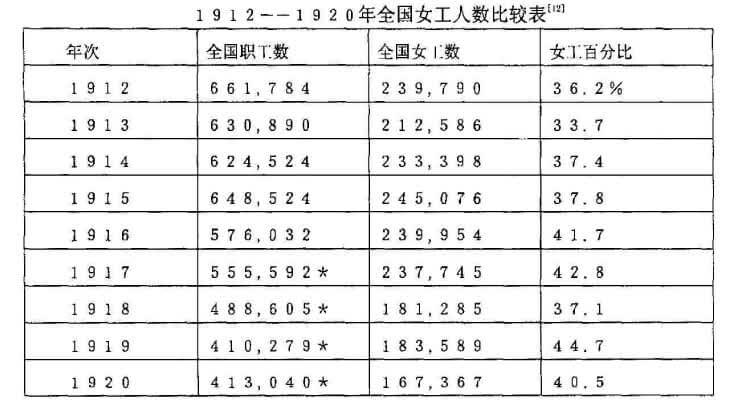
\includegraphics[width=.8\textwidth]{../docs/img/1-1.jpg}
        \caption{来源《农商统计表》第九次}
    \end{figure}
\end{frame}

\begin{frame}{西方“自然法权”和“天赋人权”思潮的输入}
    \begin{block}{}
        \begin{itemize}
            \item 1840年的鸦片战争,中国传统文化遭遇了“数千年来未有之变局”
            \item 有学者指出:“打破中国法文化封闭状态的急先锋,是近代来华的西方传教士”
            \item 传教士们通过广学会的翻译出版工作,介绍了伏尔泰、卢梭、孟德斯鸠、狄德罗等人的学说以及法律改革思想,宣传了人权观念、平等观念、法制观念
            \item 1843年开始,陆续有传教士宣扬并办女学堂,裨文女中是由美国基督教公理会传教土裨治文与夫人格兰德女士在上海创办的,宋庆龄的母亲就在这个学校就读
        \end{itemize}
    \end{block}
    \begin{figure}
        \centering
        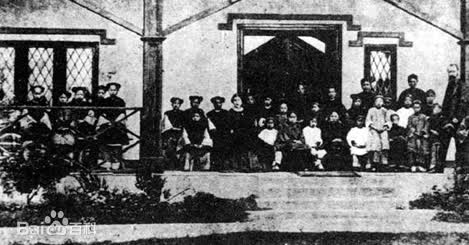
\includegraphics[height=.4\textheight]{../docs/img/1-3.jpg}
        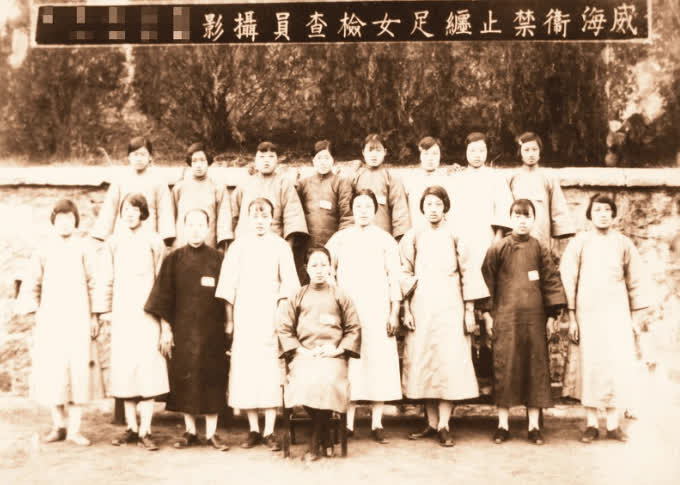
\includegraphics[height=.4\textheight]{../docs/img/1-5.jpg}
    \end{figure}
\end{frame}

\begin{frame}{西方“自然法权”和“天赋人权”思潮的输入}
    \begin{figure}
        \centering
        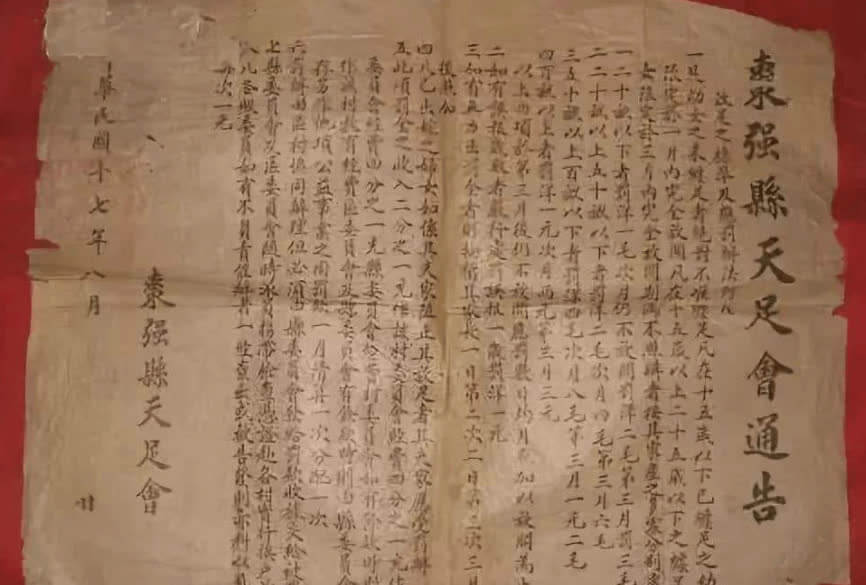
\includegraphics[height=.63\textheight]{../docs/img/1-4.jpg}
        \caption{1874年,英国传教士约翰.麦克高望率先在厦门建立了“天足会”}
    \end{figure}
\end{frame}

\begin{frame}{马克思主义思想的传入}
    \begin{block}{}
        \begin{itemize}
            \item 五四时期的一些学者将马克思主义带入了中国,随着马克思主义在中国的传播,其中有关女性的思想也在中国传播开来
            \item 出现了一系列报道女性解放运动、解读女性内心、为女性争取权益和要求改变当下女性生活现状的报纸刊物,以专栏的形式针对女性相关话题与社会大众共同探讨
            \item 女权思想也被具体化为平等地接受教育、个人的婚恋自由、独立的人格进行社会交往、经济独立等
        \end{itemize}
    \end{block}
\end{frame}

\begin{frame}{先进知识分子的推动}
    \begin{block}{}
        2019年4月30日,习近平总书记在纪念五四运动100周年大会上指出:“五四运动前后,我国一批先进知识分子和革命青年,在追求真理中传播新思想新文化,勇于打破封建思想的桎梏。”
    \end{block}
    \begin{block}{}
        \begin{itemize}
            \item 郑观应:民受生于天。天赋之以能力,使之博硕丰大,以遂其生,于是有民权焉。民权者,君不能夺之臣,父不能夺之子,兄不能夺之弟,夫不能夺之妇;
            \item 康有为:大同之世,天下为公,无有阶级,一切平等;
            \item 李大钊同志率先将马克思主义带入中国,并把唯物史观用于女权思想,让马克思主义妇女理论在中国得到了传播并开始被接受;
            \item 陈独秀曾他的文章中对“三纲五常”这一封建观念大肆鞭挞,倡导尊重个人独立自主的人格,女性要从对男性的依附中脱离出来;
            \item 鲁迅通过他的作品揭露封建社会中男女不平等的现象,严肃批判了当时社会中男性霸权对女性产生的压迫和伤害;
        \end{itemize}
    \end{block}
\end{frame}



\subsection{女权思想的主要表现}
\begin{frame}{争取受教育权}
    \begin{block}{}
        \begin{itemize}
            \item 在封建社会中,认为女子应该无才,女性不用学习文化知识,就算有部分女性能够接受教育,也是旧式教育,总是绕不开三纲五常、三从四德
            \item 近代女子学堂的开办就在新文化运动中艰难地开创起来,但上层社会人民生活的一个重要表现与欧美国家接轨,他们对女性的生活、权利、能力有了肯定和接受,并且愿意让其接受更深层次的教育
            \item 随着女子教育的振兴,使一批没有受教育权利和机会的妇女走出闺阁,接触社会,认识社会,为妇女参加政治、经济、文化活动,提高社会地位开辟了道路
        \end{itemize}
    \end{block}
    \begin{center}
        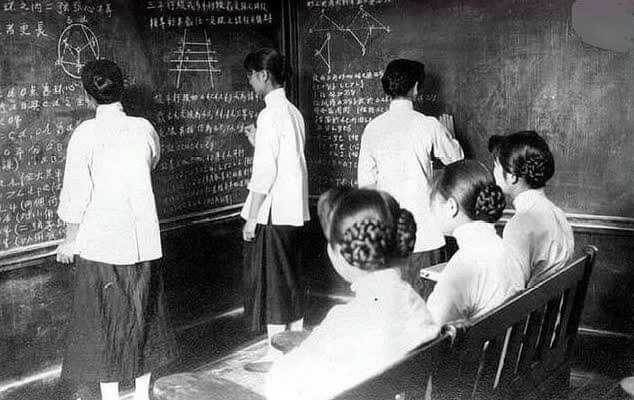
\includegraphics[width=.35\textwidth]{../docs/img/1-6.jpg}
    \end{center}
\end{frame}

\begin{frame}{争取受教育权}
    \begin{block}{}
        新文化运动以及之后女性自主性地在全国范围内倡导女权,却也只是在上层社会中适用,广大妇女仍是在艰辛地生活着和被压迫地存在着,她们没有受教育权
    \end{block}
    \begin{figure}
        \centering
        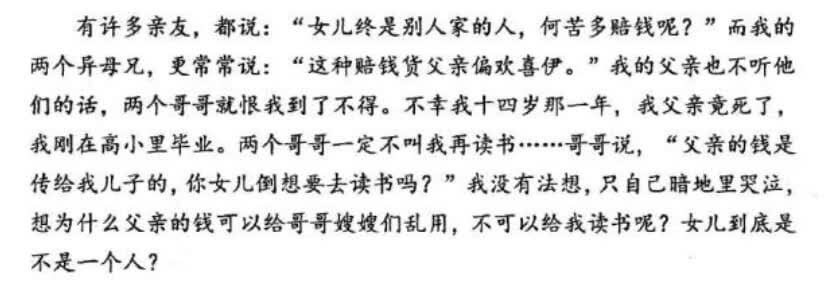
\includegraphics[width=\textwidth]{../docs/img/1-7.jpg}
        \caption{《觉悟》,1920年8月29日,第4页}
    \end{figure}
\end{frame}

\begin{frame}{争取婚姻自由权}
    \begin{block}{}
        \begin{itemize}
            \item 五四时期,先进知识分子对西方的自由婚姻观念十分推崇,他们反对包办婚姻,向封建婚姻发起了挑战
            \item 女性需要有自主选择的权利,尤其是在婚姻方面,不能再以“父母之命、媒妁之言”来束缚女性,剥夺她们婚姻自由的权利
        \end{itemize}
    \end{block}
    \begin{figure}
        \centering
        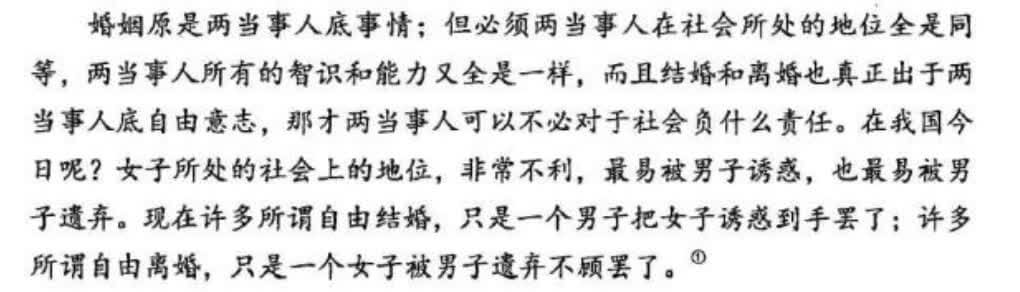
\includegraphics[width=\textwidth]{../docs/img/1-8.jpg}
        \caption{《觉悟》,1924年3月14日,第4页}
    \end{figure}
\end{frame}

\begin{frame}{争取政治参与权}
    \begin{block}{《女狱花》——王妙如}
        小说中的女主人公沙雪梅痛恨让女子受苦的社会现实,读了斯宾塞的《女权篇》,立志要改变现状。她所受的是激进女权主义的影响,以较为激烈的方式进行提倡男女平等和女子参与政权。她挑战的是整个男性社会,她将男性和女性完全对立起来,认为男人是敌人,是压迫者,而女人是被压迫者,因而提出要向男性革命。
    \end{block}
    \begin{block}{}
        \begin{itemize}
            \item 女性参政成为女性解放的重要标志,新文化运动时期的女性争取参政的运动,开始注重将其作为女性承担对于国家的责任和实现自我社会价值的重要途径
            \item 女性参政,通过获得政治上的权利来解除种种不平等的待遇,恢复天赋的人权,而且女性参与政治事务管理也是尽国民应尽的义务
        \end{itemize}
    \end{block}
\end{frame}
